Inflectional morphology in nouns is very simple.
Definiteness, gender, number, and case are not marked.

Stance forms are the main form of inflectional morphology for nouns.
They are used instead of adpositions,
and have a unique mechanism that I am not aware of in any natural language.

\subsection{Inspiration for Stance Forms}\label{subsec:inspiration-for-stance-forms}

While browsing Wikipedia at one point,
I learned that some languages, most notably in the Semitic branch,
have a ``construct state''
which involves modifying a noun to indicate
that it is possessed by another noun.
In Arabic, this process is called \textit{iḍāfah}.
One example Wikipedia gives in Egyptian Arabic is
\begin{center}
    \begin{tabular}{|c|c|}
        \hline
        malika    & a queen              \\
        \hline
        il-malika & the queen            \\
        \hline
        malik(i)t & a/the queen of \dots \\
        \hline
    \end{tabular}
\end{center}
((i) is present or absent according to sandhi.)

I found this translation with ``of \dots'' unusual
and decided it would be interesting to generalize this to
positional as well as possessive relationships.
When relating some noun (or noun phrase) to some location (or possessor),
rather than keeping the noun the same
and attaching an adposition to the location,
I will modify the noun and keep the location the same.
As far as I'm aware, no natural language does this,
so I get to invent terminology!
I call the modification of the noun a ``stance form'',
since it indicates how the noun is positioned,
which is a ``stance'' in a sense.

\subsection{Inspirational for Dimensional Distinction}\label{subsec:inspirational-for-dimensional-distinction}

I also decided that since birds can fly,
they live more three-dimensional lives than humans.
Then, it is plausible that they would have
more nuanced positional relations than humans,
including a distinction between three-dimensional ``in'' and ``on''
and two-dimensional ``in'' and ``on''.
For example,
there may be walnuts three-dimensionally in a loaf of banana bread,
while Rome is two-dimensionally in Italy (as on a map).

One source of inspiration for this is that in middle school,
I got a 3D chess variant called YAVOCH\@.
The lore in YAVOCH is that aliens are confronting humans
and have given humans spaceships to allow a fair fight.
Humans were unable to pilot the spaceships until
they connected animal brain patterns to the systems.
In particular, the animal brains (including birds)
were better with 3D spatial movement than human logic was.

There was also a time in a math class long ago when the teacher
referenced a point ``on'' a circle, meaning on the outline,
but many students assumed it was an interior point.
I thought it would be interesting to have a distinction.

\subsection{Usage of Stance Forms}\label{subsec:usage-of-stance-forms}

Stance forms will cover the following semantic roles,
with corresponding English forms:
\begin{itemize}
    \item
    Location of being
    \begin{itemize}
        \item 2D in, 2D on, 3D in, 3D on
        \item over, under, near, far from
    \end{itemize}
    \item
    Location of motion, as origin, destination, or path
    \begin{itemize}
        \item 2D into, onto, out of, off of, through, across, and 3D \dots
        \item towards, away from
    \end{itemize}
    \item
    Possession
\end{itemize}

Stance forms can also be used with partial nouns,
like ``top'' or ``side'',
which each are connected to their own nouns as possessed forms.
The same partial noun can take on different meanings according to 2D or 3D interpretation.
This can lead to very detailed descriptions of position or movement,
such as going up a mountain to reach its top face (2D ``top''),
vs.\ going up a mountain to fly in the space at its peak (3D ``top'').

Using a stance form without a verb will translate to
locational ``be'', ``go'', or possession,
according to the meaning of the stance form.
This can be thought of as a form of null copula.

The specific morphology of stance forms will be a simple suffix clitic.
The syntax is that the location (or possessor) will come first,
and the noun with the stance form will come second.

\newpage

\subsection{Examples}\label{subsec:examples2}

\begin{exe}
    \ex
    \glt
    hlātu gòna
    \glll
    hlātu gò=na \\
    plate fruit=\AdessTwo{} \\
    plate fruit=on \\
    \glt
    The fruit is on (2D) the plate.
\end{exe}

\begin{figure}[ht]
    \caption*{(4) Considering the plate as a two-dimensional region, the fruit is on the edge.}
    \centering
    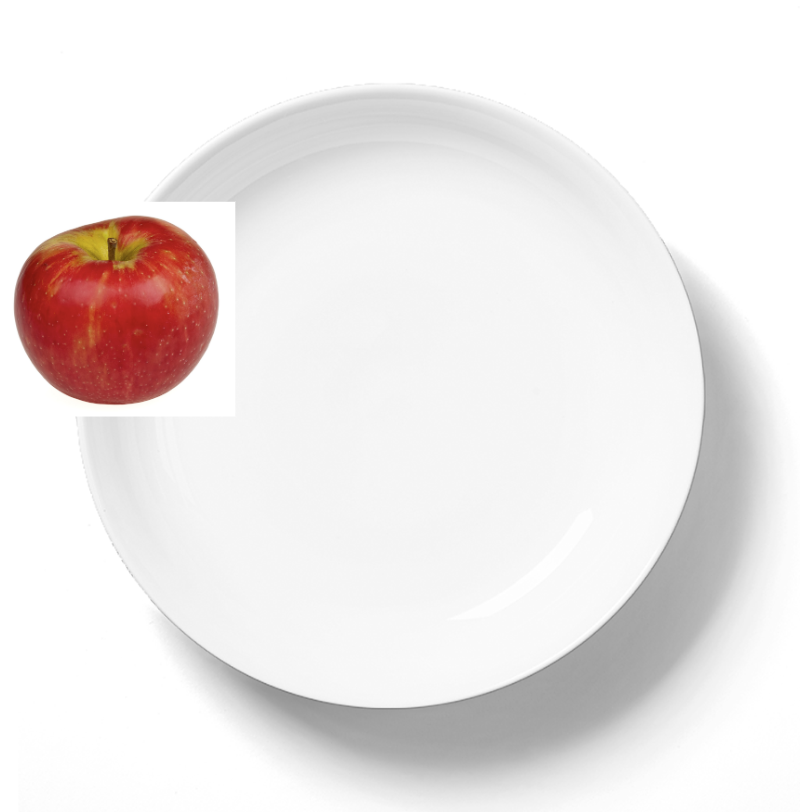
\includegraphics[scale=0.3]{adess2}\label{fig:figure2}
\end{figure}

\begin{exe}
    \ex
    \glt
    hlātu gòni
    \glll
    hlātu gò=ni \\
    plate fruit=\InessTwo{} \\
    plate fruit=in \\
    \glt
    The fruit is in (2D) the plate.
\end{exe}

\begin{figure}[ht]
    \caption*{(5) Considering the plate as a two-dimensional region, the fruit is in the interior.}
    \centering
    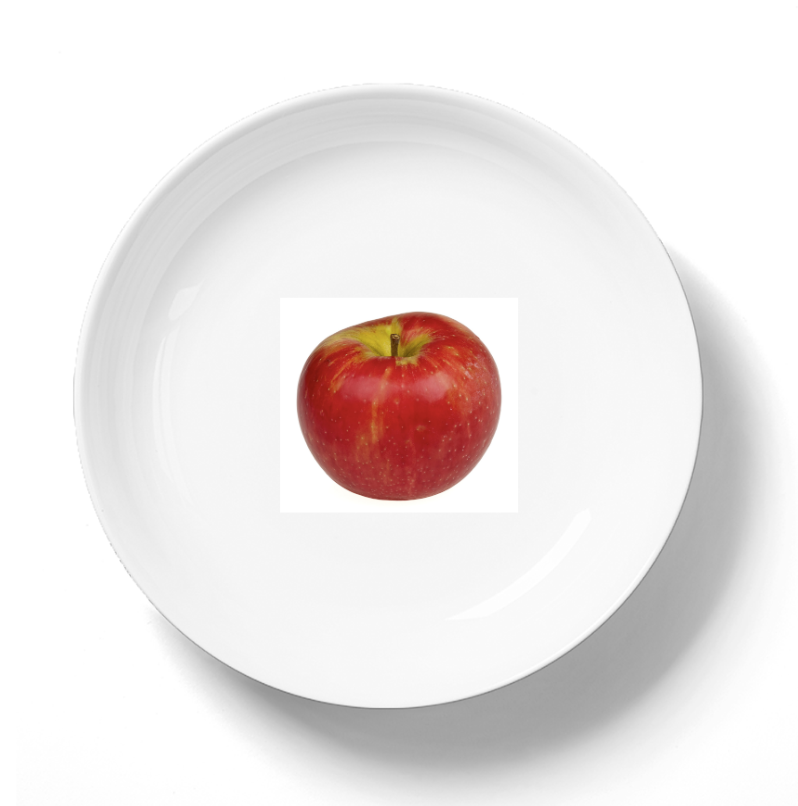
\includegraphics[scale=0.3]{iness2}\label{fig:figure3}
\end{figure}

\newpage

\begin{exe}
    \ex
    \glt
    hlātu gòla
    \glll
    hlātu gò=la \\
    plate fruit=\AdessThree{} \\
    plate fruit=on \\
    \glt
    The fruit is on (3D) the plate.
\end{exe}

\begin{figure}[ht]
    \caption*{(6) Considering the plate as a three-dimensional object, the fruit is at the exterior.}
    \centering
    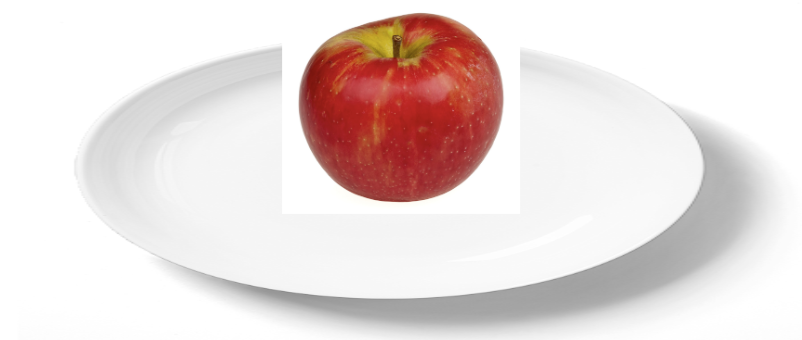
\includegraphics[scale=0.3]{adess3.1}\label{fig:figure4}
\end{figure}

\begin{figure}[ht]
    \caption*{(6) Again considering the plate as a three-dimensional object, the fruit is painted onto the exterior.}
    \centering
    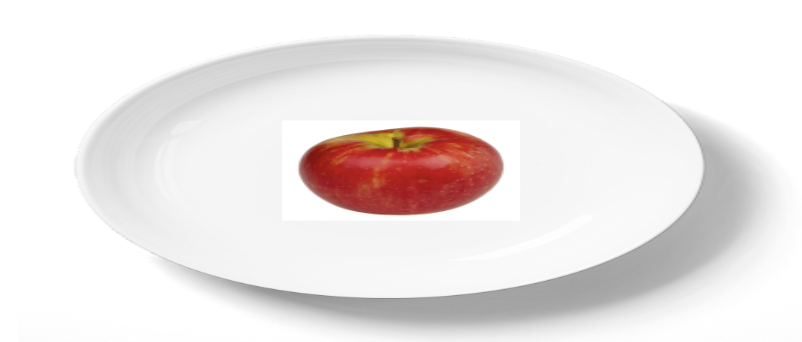
\includegraphics[scale=0.3]{adess3.2}\label{fig:figure5}
\end{figure}

\begin{exe}
    \ex
    \glt
    hlātu gòli
    \glll
    hlātu gò=li \\
    plate fruit=\InessThree{} \\
    plate fruit=in \\
    \glt
    The fruit is in (3D) the plate.
\end{exe}

\begin{figure}[ht]
    \caption*{(7) Considering the plate as a three-dimensional object, the fruit in the interior, surrounded by ceramic.}
    \centering
    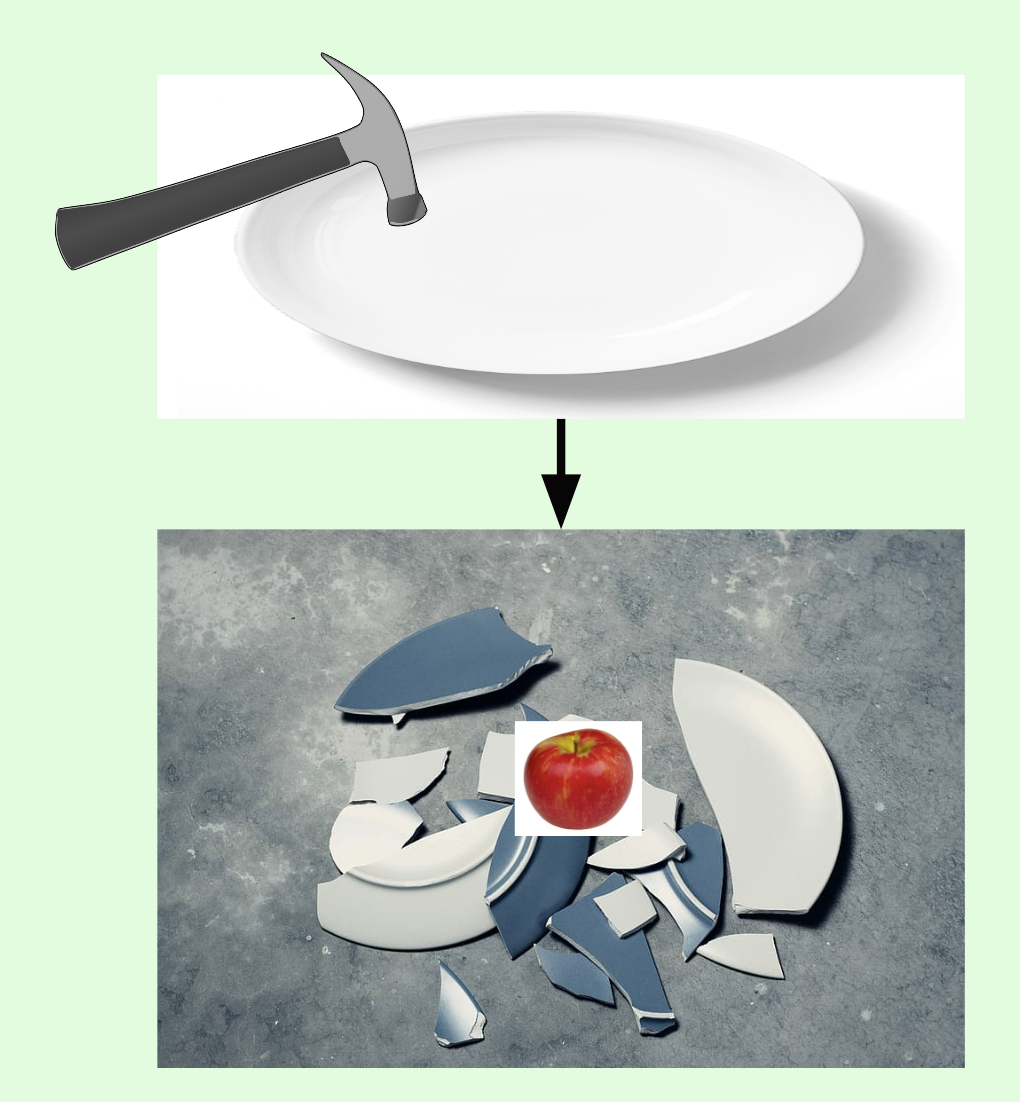
\includegraphics[scale=0.27]{iness3}\label{fig:figure6}
\end{figure}

\newpage

\begin{exe}
    \ex
    \glll
    hengó wùg=ni \\
    forest 1\Sg{}=\InessTwo{}\\
    forest I=in \\
    \glt
    I am in the forest.
\end{exe}

Large areas like forests and countries are considered two-dimensional
since they cover a flat area of the earth.

\begin{exe}
    \ex
    \glll
    rõk kwałŷx=la wùg lelō=ty=li \\
    mountain tree=\AdessThree{} 1\Sg{} nest=\Poss{}=\InessThree{} \\
    mountain tree=on I nest=\Poss{}=in \\
    \glt
    My nest is in the tree on the mountain.
\end{exe}

Trees and mountains are considered three-dimensional.
Nestled stance phrases behave as expected.
Here, ``nest'' is part of two stance phrases,
one of possession and one of location.
The stance suffixes are placed one after the other,
and the corresponding nouns are determined by order and context.

\begin{exe}
    \ex
    \glll
    kwałŷx xâr=ty słygiz=la \\
    tree top=\Poss{} vine=\AdessThree{} \\
    tree top=\Poss{} vine=towards \\
    \glt
    The vine goes up the tree.
    \ex
    \glll
    crizǐ xâr=ty słygiz=na \\
    house top=\Poss{} vine=\AdessTwo{} \\
    house top=\Poss{} vine=towards \\
    \glt
    The vine goes up the house.
\end{exe}

When a vine goes up a tree,
it grows outwards in the space near the top of the tree,
spreading in all directions.
When a vine goes up a house,
it lays flat on the roof,
restricted to the plane the roof is in.
So, ``top'' is used as 3D for the example with the tree,
and as 2D for the example with the house.

